\chapter{Building a Data-Parallel Monte Carlo Probability Estimator}
\label{chap:mc_solver}

To handle massively parallel Monte Carlo evaluations of large-scale Boolean functions, we have developed a preliminary layered architecture that organizes computation in a topological graph. At the lowest level, each Boolean variable/basic event (e.g., a component failure) is associated with a random number generator to sample its truth assignment. We bit-pack these outcome, storing multiple Monte Carlo samples in each machine word to maximize computational throughput and reduce memory footprint. Subsequent layers consist of logically higher gates or composite structures that receive the bit-packed results from previous layers and combine them in parallel using coalesced kernels. By traversing the computation graph topologically, dependencies between gates and events are naturally enforced, so kernels for each layer can run concurrently once all prerequisite layers finish, resulting in high kernel occupancy and predictable throughput.

Section~\ref{sec:kernel_execution_model} formalizes how these kernels map the logical sampling workload onto a three–dimensional ND–range, introducing a consistent coordinate system $(i_x,i_y,i_z)$ and a rounding scheme that guarantees complete coverage without redundancy.  The remainder of this chapter adopts that notation.

In practice, each layer is dispatched to an accelerator node using a data-parallel model implement using \acrshort{sycl}. The random number generation pipelines are counter-based, ensuring reproducibility and thread-safety even across millions or billions of samples. Gates that go beyond simple AND/OR logic--such as \acrshort{vot} operators--are handled by specialized routines that can exploit native popcount instructions for efficient threshold evaluations. As we progress upwards through the layered topology, each gate or sub-function writes out its bit-packed output, effectively acting as an input stream to the next layer.
Throughout the simulation, online tallying kernels aggregate how often each node or gate evaluates to True. These tallies can then be turned into estimates of probabilities and sensitivity metrics on the fly. This approach also makes adaptive sampling feasible: if specific gates appear to dominate variance or are tied to particularly rare events, additional sampling can be allocated to their layer to refine estimates.


\section{Layered Topological Organization}
\label{sec:layered_dag_traversal}

Recall that a \acrshort{pdag} \(\mathcal{G} = (\mathcal{V}, \mathcal{E})\) contains no cycles, so there is at least one valid \emph{topological ordering} of its nodes.  A topological ordering assigns each node a numerical \emph{layer index} such that all edges point from a lower-numbered layer to a higher-numbered layer. If a node \(v\) consumes the outputs of nodes \(\{u_1,\dots,u_k\}\), then we require
\[
\text{layer}(u_i) \;<\; \text{layer}(v)
\quad
\text{for each }i\in\{1,\dots,k\}.
\]
In other words, node \(v\) can appear only after all of its inputs in a linear or layered listing.

The essential steps to build and traverse these layers are:

\begin{enumerate}
    \item \emph{Compute Depths via Recursive Analysis:}  
      Each node's depth is found by inspecting its children (or inputs).  If a node is a leaf (e.g., a \texttt{Variable} or \texttt{Constant} that does not depend on any other node), its depth is 0.  Otherwise, its depth is one larger than the maximum depth among its children.  

    \item \emph{Group Nodes by Layer:}  
      Once each node's depth is computed, nodes of equal depth form a single \emph{layer}. Thus, all nodes with depth \(0\) are in the first layer, those with depth \(1\) in the second layer, and so on.  

    \item \emph{Sort Nodes within Each Layer:}  
      Within each layer, enforce an additional consistent ordering: (i)~variables appear before gates, (ii)~gates of different types can be grouped to facilitate specialized processing.  This step is not strictly required for correctness, but it can streamline subsequent stages such as kernel generation or partial evaluations.

    \item \emph{Traverse Layer by Layer:}  
      A final pass iterates over each layer in ascending order.  Because all inputs of any node in layer \(d\) lie in layers \(< d\), the evaluation (or "kernel build") for layer \(d\) can proceed after the entire set of layers \(0,\dots,d-1\) is processed.
\end{enumerate}

This structure ensures a sound evaluation of the \acrshort{pdag}: no gate or variable is computed until after all of its inputs are finalized.

\begin{figure}
    \centering
    \begin{subfigure}{1\textwidth}
        \centering
        \includesvg[height=0.3\textheight]{figs/pdag/dag_pass_1.svg}
    \caption{Working example from Fig.~\ref{fig:pdag_pass_1}.}
        \label{fig:recall_pdag_pass_1}
    \end{subfigure}
    \vfill
    \begin{subfigure}{1\textwidth}
        \centering
        \includesvg[width=0.6\linewidth]{figs/pdag/dag_pass_2.svg}
        \label{fig:pdag_pass_2}
    \end{subfigure}
    \caption{Layered topological ordering on the Propositional \acrfull{dag}, with coalesced/fused kernels, partitioned by operation type.}
\end{figure}

\subsection{Depth Computation and Node Collection}

\begin{enumerate}
    \item \textbf{Clear Previous State.}  
      Any existing "visit" markers or stored depths in the \acrshort{pdag}-based data structures are reset to default values (e.g., zero or -1).
      
    \item \textbf{Depth Assignment by Recursion.}  
      A \texttt{compute\_depth} subroutine inspects each node:
      \begin{enumerate}
        \item If the node is a \texttt{Variable} or \texttt{Constant}, it is a leaf in the \acrshort{pdag}, so depth \(=0\).  
        \item If the node is a \texttt{Gate} with multiple inputs, the procedure first recursively computes the depths of its inputs. It then sets its own depth as 
        \[
          \text{depth}(\texttt{gate})
          \;=\;
          1 \;+\;\max\limits_{\ell \in \text{inputs of gate}} \Bigl[\text{depth}(\ell)\Bigr].
        \]
      \end{enumerate}
    \item \textbf{Order Assignment.}  
      Each node stores the newly computed depth in an internal field. This numeric value anchors the node to a layer. A consistent pass over the entire graph ensures correctness for all nodes.
\end{enumerate}

After depths are assigned, gather all nodes, walking the \acrshort{pdag} from its root, recording each discovered node and adding it to a global list.

\subsection{Layer Grouping and Local Sorting}

Begin by creating:
\begin{itemize}
\item A global list of all nodes, each with a valid depth,  
\item A mapping from node indices to node pointers,  
\end{itemize}
Then, sort the global list by ascending depth.  Let \(\text{order}(n)\) be the depth of node \(n\).  Then
\[
\text{order}(n_1)\;\le\;\text{order}(n_2)\;\le\;\dots\,\le\;\text{order}(n_{|\mathcal{V}|}).
\]
Finally, partition this list into contiguous \emph{layers}: if the deepest node has a depth \(\delta_{\max}\), then create sub-lists:
\[
\{\text{nodes s.t. depth}=0\},
\quad
\{\text{nodes s.t. depth}=1\},
\quad
\dots,
\quad
\{\text{nodes s.t. depth}=\delta_{\max}\}.
\]
Within each layer, sort nodes to ensure that \texttt{Variable} nodes precede \texttt{Gate} nodes, and \texttt{Gate} nodes may be further sorted by \texttt{Connective} type (e.g., \texttt{AND}, \texttt{OR}, \texttt{VOT}, etc.).

\subsection{Layer-by-Layer Kernel Construction}

Apply the layer decomposition to drive \emph{kernel building} and \emph{evaluation}:

\begin{enumerate}
    \item \textbf{Iterate over each layer in ascending depth}.  Because every node's dependencies lie in a strictly lower layer, one is guaranteed that those dependencies have already been assigned memory buffers, partial results, or other necessary resources.
    \item \textbf{Partition the layer nodes into subsets by node type}.  Concretely, \texttt{Variable} nodes are batched together for \emph{basic-event sampling} kernels, while \texttt{Gate} nodes are transferred into \emph{gate-evaluation} kernels.  
    \item \textbf{Generate device kernels}.  For \texttt{Variable} nodes, create Monte Carlo sampling kernels. For \texttt{Gate} nodes, it constructs logical or bitwise operations that merge or transform the sampled states of the inputs.  
\end{enumerate}

Once kernels for a given layer finish, move on to the next layer. Because of the topological guarantee, no node in layer \(d\) references memory or intermediate states from layer \(d\!+\!1\) or later, preventing cyclical references and ensuring correctness.


\section{Adopting the SYCL Execution Model}

Before getting into our opinionated launch parameters, it is instructive to recall the abstract execution hierarchy defined by the SYCL standard. This detour provides the conceptual foundation upon which the remainder of this dissertation builds.

\begin{figure}[hb]
    \centering
    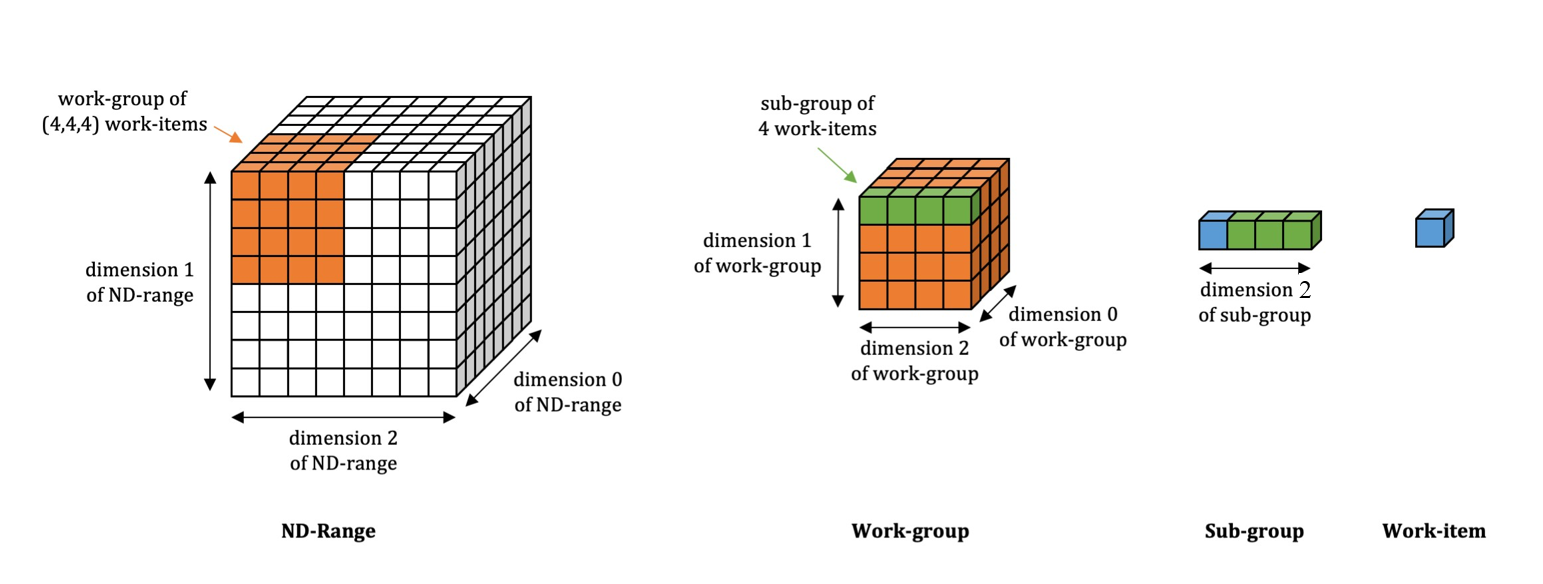
\includegraphics[width=1\textwidth]{figs/sycl/sycl_execution_model.png}
    \caption{At a glance: The SYCL execution model describes relationships between ND-Ranges, work-groups, sub-groups, and work-items.}
    \label{fig:sycl_exec_model}
\end{figure}

% -----------------------------------------------------------------------------
%  Conceptual overview and formal relationships
% -----------------------------------------------------------------------------
\subsection{Conceptual Overview}  Modern accelerator programming models must present the developer with a 
\emph{logical} view of parallel work that is independent of any specific piece of hardware.  SYCL achieves this
by defining a small hierarchy of index spaces.  Each level in the hierarchy provides progressively stronger 
coherence and synchronization guarantees, yet none of them prescribes 
\textit{where} that work will eventually run.  The mapping from logical indices to physical execution resources is
entirely deferred to the run--time or device compiler and is therefore opaque to the application.  In what follows we formalize the four key abstractions exposed by the SYCL execution model and derive a set of identities that will be reused throughout the remainder of this dissertation.

\subsection{Hierarchical Index Spaces}  Let
\[
   \mathbf{G} = (G_x,G_y,G_z) \in \mathbb{N}^3, \qquad
   G_d > 0\quad(d\in\{x,y,z\}) ,
\]
be the \emph{global range}.  It enumerates the total number of logical tasks, or \emph{work--items}, that shall be executed in one kernel invocation.  The associated set of global indices is
\[
    \mathcal{I} \;=\; \{0,\dots,G_x-1\} \times \{0,\dots,G_y-1\} \times \{0,\dots,G_z-1\},
\]
with
\( |\mathcal{I}| = G_x G_y G_z. \)

A second triple
\[
    \mathbf{L} = (L_x,L_y,L_z), \qquad 0 < L_d \le G_d ,
\]
referred to as the \emph{local range}, partitions the ND--Range into disjoint \emph{work--groups}.  Defining
\[
    W_d \;=\; \frac{G_d}{L_d},\qquad d\in\{x,y,z\},
\]
(which implies $G_d \equiv 0\; (\mathrm{mod}\,L_d)$), the set of group indices reads
\[
    \mathcal{W} \;=\; \{0,\dots,W_x-1\} \times \{0,\dots,W_y-1\} \times \{0,\dots,W_z-1\},
\]
with cardinality $|\mathcal{W}|=W_x W_y W_z$.  Each group $w\in\mathcal{W}$ owns exactly
\[
    |\Gamma| \;=\; L_x L_y L_z
\]
work--items that share fast local memory and barrier synchronization.

Within a work--group the implementation may further partition the local index space into \emph{sub--groups} of size $S$:
\[
    S \;=\; |\Sigma|,\quad \Sigma \subseteq \Gamma,\quad 1\le S\le |\Gamma|.
\]
Sub--groups execute in (near) lockstep and admit specialized collective operations, yet their existence and size remain device--specific.  Finally, the singleton element of the hierarchy is the \textbf{work--item}, uniquely addressed by its global id $i=(i_x,i_y,i_z)\in\mathcal{I}$.

The containment relations
\[
    \text{work--item} \;\in\; \text{sub--group} \;\subseteq\; \text{work--group} \;\subseteq\; \text{ND--Range}
\]
hold for every index triple.

\subsection{Abstractness of the Model}  None of the above definitions mention vector widths, cores, or memory banks.  The SYCL execution model is strictly an \emph{index algebra}; it provides (i)~a naming scheme for independent pieces of work, and (ii)~a lattice of synchronization points that the run--time must respect.  Once the tuples $\mathbf{G}$ and $\mathbf{L}$ have been fixed, every additional property of the physical execution, including occupancy, scheduling order, and even whether groups are run concurrently or serially, is an implementation detail.

\subsection*{Notation used from here onward.}  We will exploit the following shorthand throughout the subsequent analysis:
\begin{enumerate}
  \item $|\mathcal{I}|=G_xG_yG_z$ \quad (total work--items),
  \item $|\mathcal{W}|=W_xW_yW_z$ \quad (total work--groups),
  \item $|\Gamma|=L_xL_yL_z$        \quad (work--items per group),
  \item $\langle i_g,i_l\rangle$\quad embodiment of a work--item by its enclosing group index $i_g\in\mathcal{W}$ and its local index $i_l\in\Gamma$.
\end{enumerate}
These identities are purely algebraic and therefore remain valid for \emph{any} SYCL--conformant device.

\paragraph*{From Abstraction to Implementation Strategy.} Next, we translate these concepts into the concrete launch geometries and dependency patterns required by our Monte--Carlo solver.  The forthcoming sections build progressively from global range rounding rules to kernel--specific mappings.
% -----------------------------------------------------------------------------
%  Extended algorithmic description of kernel generation and execution
% -----------------------------------------------------------------------------

\subsection{Basic--Event Sampling Kernels}
\label{subsec:be_kernel}

Each \texttt{Variable} node in layer~$d$ represents an i.i.d.~Bernoulli trial
with success probability~$p\_v\in[0,1]$.  The evaluation of all variables in
a layer is consolidated into 
\emph{one} data--parallel kernel that generates a contiguous block of
bit--packed outcomes:
\begin{enumerate}
  \item \textbf{Parameter staging.}  For every variable~$v$ the solver stores the
        pair $(\text{idx}(v),\,p\_v)$ in host memory, where
        $\text{idx}(v)$ is the global node index.  The list is stable across
        Monte--Carlo iterations and is therefore transferred to device memory
        only once.
  \item \textbf{Contiguous layout.}  A device--side array of $N_{\!v}$
        records, $N_{\!v}$ being the number of variables in the layer, is
        allocated so that the probability field, the bit--packed result buffer
        pointer, and any auxiliary counters are stored in
        \emph{structure--of--arrays} (SoA) form.  The resulting stride--free
        access pattern maximizes global--memory throughput.
  \item \textbf{Kernel configuration.}  Let $T$ denote the total number of
        Bernoulli draws requested by the host run--time (cf.
        Sec.~\ref{sec:bitpack-prob-sampling}).  The global ND--range is chosen
        as $\bigl(\lceil N_{\!v}\rceil,\,B,\,P\bigr)$, mapping each work--item
        to a unique triple $(v,\,b,\,p)$ of variable~$v$, batch index~$b$, and
        bit--pack index~$p$.  The local work--group shape is computed
        adaptively to saturate the target device while respecting hardware
        limits on registers and shared memory.
  \item \textbf{Execution.}  Every work--item initializes a counter--based
        generator (see the Philox discussion in
        Sec.~\ref{sec:bitpack-prob-sampling}), converts the pseudo--random words
        into $\omega$ Bernoulli outcomes via the integer--threshold technique,
        and writes the resulting $w$--bit word to the pre--allocated buffer.
        No inter--item synchronization is required beyond the implicit barrier
        at kernel completion.
\end{enumerate}
The overall cost is $\mathcal{O}(T\,N_{\!v}/\omega)$ arithmetic operations and
$\Theta(T\,N_{\!v}/\omega)$ global writes, making the routine
memory--bandwidth bound only for extremely small~$P$.

\subsection{Gate--Evaluation Kernels}
\label{subsec:gate_kernel}

Gate nodes are logically heterogeneous: AND, OR, XOR, NOT, NAND, NOR, XNOR, and
at--least--$k$ (\texttt{VOT}) gates all feature distinct Boolean semantics yet
share the same interface of reading one or more bit--packed input buffers and
writing a bit--packed output.  To avoid divergent control flow, the solver
instantiates \emph{one specialized kernel per connective type} present in the
current layer.

Consider a set $\mathcal{G}_{\mathrm{type}}$ containing all gates of a single
connective.  Their evaluation proceeds as follows:
\begin{enumerate}
  \item \textbf{Input resolution.}  For every gate $g\in\mathcal{G}$ the lists
        of positive inputs $\mathcal{I}^+(g)$ and negated inputs
        $\mathcal{I}^-(g)$ are resolved to concrete device pointers.  Positive
        and negative buffers are concatenated so that a simple offset marks the
        first negated operand.  The construction is embarrassingly parallel on
        the host and involves no device work.
  \item \textbf{Contiguous block construction.}  Buffers and gate metadata are
        packed into an SoA structure that is tile--aligned for
        coalesced reads.  For at--least--$k$ gates the threshold~$k$ is stored
        alongside the pointer list.
  \item \textbf{Kernel launch geometry.}  Let $N_{\!g}$ be the number of gates
        of the selected type.  An ND--range of
        $\bigl(\lceil N_{\!g}\rceil,\,B,\,P\bigr)$ is created, identical in
        shape to the basic--event kernel so that subsequent layers can reuse
        the same scheduling heuristics.  Within each work--item, Boolean logic
        is applied on a per--bitpack basis without branching:
        \begin{itemize}
          \item \textsc{And}, \textsc{Nand}:  multiple \texttt{\&} reductions
                plus an optional complement.
          \item \textsc{Or}, \textsc{Nor}:   multiple \texttt{|} reductions
                plus an optional complement.
          \item \textsc{Xor}, \textsc{Xnor}: accumulated parity via \texttt{\^{}} operations.
          \item \textsc{Null}, \textsc{Not}: trivial one--input, output, with complement.
          \item \textsc{At--least--$k$}: population counting of the aggregated
                bit--wise sum followed by a threshold comparison implemented
                through native \texttt{popcount} instructions.
        \end{itemize}
  \item \textbf{Dependency guarantees.}  Because all input buffers originate in
        earlier layers, the run--time enforces an event dependency on every
        producing kernel, ensuring visibility of the complete inputs before
        gate evaluation begins.
\end{enumerate}
The bit--parallel operations ensure that the arithmetic intensity is high; the
critical path is dominated by a handful of integer masks and, for
at--least--$k$ gates, one integer addition plus a comparison per input.

\subsection{Dependency--Aware Kernel Scheduling}
\label{subsec:scheduling}

Kernels are submitted to the device queue in strict layer order, yet the
scheduler exploits two orthogonal forms of parallelism:
\begin{enumerate}
  \item \emph{Intra--layer concurrency} --- basic--event sampling and the
        multiple gate kernels of the same layer depend exclusively on the
        previous layer, \emph{not} on one another.  They are therefore eligible
        for concurrent execution subject to device resources.
  \item \emph{Iterative sampling} --- the bit--packed sample space is sliced
        into $T_\text{iter}$ iterations decided by the sample shaper.
        Kernels capturing the same node repeat across iterations and are
        expressed with an explicit iteration counter, enabling the run--time to
        re--use the same compiled binary while varying the random counter seed
        and output offsets.
\end{enumerate}
Dependencies are represented as light--weight events; the host never performs
explicit synchronization inside a layer but relies on the queue to enforce the
partial order.

\subsection{Work--Group Optimization Heuristics}
\label{subsec:wg_optim}

Let $G$ denote the global item count of the kernel at hand and $L_{max}$ the
maximum local size supported by the device along each axis.  The solver
selects a local range $(l_x,l_y,l_z)$ according to
\begin{align*}
  l_x &= min\Bigl(\text{pow2ceil}(G),\,L_{max}\Bigr),\\
  l_y &= min\Biggl(B,\,\frac{L_{max}}{l_x}\Biggr),\\
  l_z &= min\Biggl(P,\,\frac{L_{max}}{l_x l_y}\Biggr),
\end{align*}
which heuristically balances occupancy with register pressure while retaining a
uniform work--item distribution.  The shape is re--evaluated independently for
basic events and gate kernels because $G$ differs across those two categories.

\subsection{Complexity and Scalability}
\label{subsec:complexity}

Assume $|\mathcal{V}|$ variables and $|\mathcal{G}|$ gates in the graph, with
layer depths bounded by $D$.  Let $S=T\,B\,P\,\omega$ be the total number of
Bernoulli trials.
\begin{itemize}
  \item \textbf{Kernel build time.}  All host--side preprocessing runs in
        $\mathcal{O}(|\mathcal{V}|+|\mathcal{G}|)$ memory operations; no search
        structure deeper than a hash map is required.
  \item \textbf{Device execution time.}  Each basic--event kernel performs
        $S$ integer comparisons.  Each gate kernel evaluates $S$ Boolean
        operations whose count is proportional to the fan--in of the gate.
        Hence the total arithmetic complexity is
        $\mathcal{O}\bigl(S\,(1+\overline{\deg})\bigr)$, where
        $\overline{\deg}$ is the average gate fan--in.
  \item \textbf{Parallel scalability.}  Both kernel categories exhibit linear
        speed--up with the number of compute units until either (i)~the global
        launch size no longer saturates the device or (ii)~memory bandwidth
        limits are reached.  Because all kernels are fully independent across
        the $B$ and $P$ dimensions, they scale particularly well on
        multi--tile accelerators.
\end{itemize}

The design therefore provides a clear separation of concerns: depth--first
analysis establishes the dependency structure; kernel generation translates
that structure into homogeneous, vectorizable work; and a light--weight event
system schedules the resulting kernels with minimal host intervention.


\begin{landscape}
\begin{figure}[p]
    \centering
    \includesvg[width=1.15\textheight]{figs/pdag/dag_pass_3.svg}
    \caption{A fully connected Probabilistic-Propositional Directed Acyclic Graph.}
    \label{fig:feedforward_ppdag}
\end{figure}
\end{landscape}


% -----------------------------------------------------------------------------
\section{Kernel-Level Execution Model}
\label{sec:kernel_execution_model}
% -----------------------------------------------------------------------------

\subsection{Coordinate System and Notation}

Let $(G_x,G_y,G_z)\in\mathbb{N}^3$ denote the \emph{global} range supplied to the device and $(L_x,L_y,L_z)$ the \emph{local} (work\,–\,group) range.  We further define
\[
  W_d \;=\; \frac{G_d}{L_d},\qquad d\in\{x,y,z\},
  \quad\text{and}\quad
  W \;=\; W_x W_y W_z ,
\]
where $W_d$ counts work-groups along axis~$d$ and $W$ is the total number of work-groups.  Every work-item within a group is identified by its local id $\ell=(\ell_x,\ell_y,\ell_z)$ with $0\le \ell_d<L_d$.

Unless stated otherwise the following global symbols are used throughout the chapter
\begin{center}
\begin{tabular}{ll}
$V$  & \# basic events (variables)\\
$G$  & \# standard logic gates\\
$A$  & \# at-least-$k$ gates\\
$T$  & Monte-Carlo iterations\\
$B$  & batches per iteration\\
$P$  & bit-packs per batch\\
$\omega$ & bits per pack $=8\cdot\mathrm{sizeof}(\texttt{bitpack\_t})$\\
$N$  & trials per iteration $=B\,P\,\omega$
\end{tabular}
\end{center}

\subsection{Generic Rounding Scheme}

All kernels adopt the \emph{nearest-multiple} rule
\[
   G_d \;=\;
   \Bigl\lceil \frac{Q_d}{L_d} \Bigr\rceil L_d ,\qquad
   Q_d \in \{V,G+A,1\}\times\{B\}\times\{P\},
\]
where $Q_d$ is the problem-specific lower bound listed in Table~\ref{tab:kernel_dimensions}.  This rule guarantees that every logical task is scheduled while respecting the SYCL constraint $G_d\equiv 0 \; (\mathrm{mod}\,L_d)$.

\subsection{Kernel-Specific Mappings}

Each kernel instantiates a surjective mapping
\[
   \Phi : \{0,\dots,G_x-1\}\times\{0,\dots,G_y-1\}\times\{0,\dots,G_z-1\}
          \;\twoheadrightarrow\; \mathcal{S},
\]
where $\mathcal{S}$ is the set of logical sub-tasks it must solve.  We list the mappings succinctly:

\begin{itemize}
  \item \textbf{Basic-event sampling} ($\#\mathcal{S}=VBP$):
        $\,\Phi_{\mathrm{BE}}(i_x,i_y,i_z)=(v=i_x,\;b=i_y,\;p=i_z)$.

  \item \textbf{Standard gate evaluation} ($\#\mathcal{S}=GBP$):
        $\,\Phi_{\mathrm{G}}(i_x,i_y,i_z)=(g=i_x,\;b=i_y,\;p=i_z)$.

  \item \textbf{At-least-$k$ gate evaluation}
        ($\#\mathcal{S}=ABP\omega$):
        $\,i_z = p\,\omega + \lambda$ with $\lambda\in\{0,\dots,\omega-1\}$.  The pair $(b,p)$ indexes the bit-pack, while $\lambda$ singles out a \emph{bit lane}.  One work-group therefore owns a unique triplet $(a,b,p)$ and folds the $\omega$ lanes with a group reduction.

  \item \textbf{Tally accumulation} ($\#\mathcal{S}=VBP$):
        identical to $\Phi_{\mathrm{BE}}$ but with $L_x=1$ such that each group covers exactly one tally node.
\end{itemize}

\subsection{Trial Coverage Guarantee}

Let $\Xi$ be the set of Bernoulli trials processed by a kernel in one iteration.  By construction
\[
   |\Xi|
   \;=\;
   \underbrace{B P \omega}_{\text{trials/ node}}
   \times
   \begin{cases}
     V, & \text{basic-event},\\[2pt]
     G, & \text{standard gate},\\[2pt]
     A, & \text{at-least gate},\\[2pt]
     V, & \text{tally}.
   \end{cases}
\]
Because $\omega$ divides $G_z$ in every case, each trial is owned by exactly one work-item and is executed precisely once.

\begin{table}[t]
  \centering
  \caption{Minimum global dimensions $Q_d$ before round-up.}
  \label{tab:kernel_dimensions}
  \begin{tabular}{lccc}
    \toprule
    Kernel               & $Q_x$              & $Q_y$ & $Q_z$\\
    \midrule
    Basic-event          & $V$                & $B$   & $P$\\
    Standard gate        & $G$                & $B$   & $P$\\
    At-least-$k$ gate    & $A$                & $B$   & $P\omega$\\
    Tally                & $V$                & $B$   & $P$\\
    \bottomrule
  \end{tabular}
\end{table}

\subsection{Work-Group Invariants}

Let $\Gamma$ be a work-group.  For every kernel the following invariant holds inside $\Gamma$:
\[
   \bigl[(\ell_x,\ell_y,\ell_z)\in\Gamma\bigr]
   \;\Longrightarrow\;
   \text{all work-items share the complete set of inputs required to produce one output literal}.
\]
Consequently intra-group communication (reductions, barriers) never crosses logical boundaries, enabling lock-free execution except for the single atomic update in the tally kernel.

\subsection{Complexity per Work-Group}

With $L=L_xL_yL_z$ the number of instructions executed by a group is
\[
  C_{\Gamma}
  \;=\;
  \begin{cases}
    \Theta(\frac{\omega}{4}), & \text{basic-event (bit-packing)},\\
    \Theta(\deg g), & \text{gate of fan-in }\deg g,\\
    \Theta(\deg a + \log \omega), & \text{at-least-}k,\\
    \Theta(L + \log L), & \text{tally popcount + reduction},
  \end{cases}
\]
all independent of $T$ owing to the strict buffering between iterations.

% -----------------------------------------------------------------------------
\section{Bitpacked Random Number Generator}

Monte Carlo simulations, probability evaluations, and other sampling-based procedures benefit greatly from efficient, high-quality \acrfull{rng}s. A large class of modern \acrshort{rng}s are known as \textit{counter-based \acrfull{prng}s}, because they use integer counters (e.g., 32-bit or 64-bit) along with a stateless transformation to produce random outputs. The \emph{Philox} family of counter-based \acrshort{prng}s is a well-known example, featuring fast generation, high period, and good statistical properties. In this section, we discuss the general principles of counter-based \acrshort{prng}s, explain how Philox fits into this paradigm, analyze its complexity, and present a concise pseudocode version of the \(\text{Philox }4\times32\text{-10}\) variant. Subsequently, we detail the bitpacking scheme used to reduce memory consumption when storing large numbers of Bernoulli samples.

A counter-based \acrshort{prng} maps a user-supplied \emph{counter} (plus, optionally, a \emph{key}) to a fixed-size block of random bits via a deterministic function. Formally, if 
\[
  \mathbf{x} \;=\; (x_1, x_2, \ldots, x_k)
\]
is a vector of one or more 32-bit or 64-bit counters, and 
\[
  \mathbf{k} \;=\; (k_1, k_2, \ldots, k_m)
\]
is a key vector, then a counter-based \acrshort{prng} defines a transformation 
\[
   \mathcal{F}(\mathbf{x}, \mathbf{k})
   \;=\;
   (\rho_1, \rho_2, \ldots, \rho_r),
\]
where each \(\rho_j\) is typically a 32-bit or 64-bit output. Different increments of the counter \(\mathbf{x}\) produce different pseudo-random outputs \(\rho_j\). The process is stateless in the sense that advancing the RNG amounts to incrementing the counter (e.g., \(\mathbf{x}\mapsto \mathbf{x} + 1\)).

Compared to older recurrence-based \acrshort{rng}s such as linear congruential generators or the Mersenne Twister, counter-based methods offer more straightforward parallelization, reproducibility across multiple streams, and strong structural simplicity: no internal state must be updated or maintained. This is particularly valuable in distributed Monte Carlo simulations or \acrshort{gpu}-based sampling, where each thread or work-item can be assigned a different counter. Philox constructs its pseudo-random outputs by applying a small set of mixed arithmetic (multiplication/bitwise) rounds to an input \emph{counter} plus \emph{key}. In particular, \(\mathrm{Philox}\,4\times32\text{-10}\) (often shortened to "Philox-4x32-10”) works on four 32-bit integers at a time:
\[
  \mathbf{S} = (S_0, S_1, S_2, S_3),
  \qquad
  \mathbf{K} = (K_0, K_1).
\]
The four elements \(\{S_0, S_1, S_2, S_3\}\) collectively represent the counter, e.g., \((x_0, x_1, x_2, x_3)\). The two key elements \((K_0, K_1)\) are used to tweak the generator's sequence. A single invocation of Philox-4x32-10 transforms \(\mathbf{S}\) into four new 32-bit outputs after ten rounds of mixing. At each round, the algorithm:
\begin{enumerate}
    \item Multiplies two of the state words by fixed "magic constants” to create partial products.
    \item Takes the high and low 32-bit portions of those 64-bit products.
    \item Incorporates the round key to shuffle the words.
    \item Bumps the key by adding constant increments \((\mathrm{W32A} = 0x9E3779B9 \text{ and } \mathrm{W32B} = 0xBB67AE85)\).
\end{enumerate}
After ten rounds, the final \((S_0, S_1, S_2, S_3)\) is returned as the pseudo-random block. A new call to Philox increases the counter \(\mathbf{S}\) by one (e.g., \(S_3 \mapsto S_3 + 1\)) and re-enters the same function. The Philox-4x32-10 algorithm is designed so that each blocking call requires a \emph{constant number} of operations, independent of the size of any prior "state.” Specifically, each round involves:
\[
  \mathcal{O}(1)\;\text{ arithmetic operations},
\]
and there are \(\mathrm{R} = 10\) rounds. Thus, each Philox invocation is asymptotically constant time \(\mathcal{O}(\mathrm{R}) = \mathcal{O}(1)\). The total cost to generate 128 bits (4 words \(\times\) 32 bits) is therefore constant time per call.

\subsection{The 10-round Philox-4x32}
Our implementation follows the standard 10-round approach for generating one block of four 32-bit random words, also called Philox-4x32-10. Let \(M_{\mathrm{A}}=0xD2511F53\), \(M_{\mathrm{B}}=0xCD9E8D57\) be the multipliers, and let \((K_0, K_1)\) be the key which is updated each round by \(\mathrm{W32A}=0x9E3779B9\) and \(\mathrm{W32B}=0xBB67AE85\). The function \(\text{Hi}(\cdot)\) returns the high 32 bits of a 64-bit product, and \(\text{Lo}(\cdot)\) returns the low 32 bits. Because each call produces four 32-bit pseudo-random words, Philox-4x32-10 is particularly convenient for batched sampling. If only a single 32-bit word is needed, one can still call the function and discard the excess words; however, many applications consume all four outputs (e.g., to produce four floating-point variates).

\begin{algorithm}[ht]
  \caption{Philox-4x32-10}\label{alg:philox}
  \begin{algorithmic}[1]
    %------------------------------------------------------------
    \Require Four 32-bit counters $(S_0,S_1,S_2,S_3)$,
            key $(K_0,K_1)$
    \Ensure  Transformed counters $(S_0,S_1,S_2,S_3)$
    %------------------------------------------------------------
    \Statex
    %--------------------- Philox_Round -------------------------
    \Procedure{Philox\_Round}{$(S_0,S_1,S_2,S_3),\,(K_0,K_1)$}
      \State $P_0 \gets M_{\text{A}}\times S_0$ \Comment{64-bit product}
      \State $P_1 \gets M_{\text{B}}\times S_2$ \Comment{64-bit product}
      \State $T_0 \gets \mathrm{Hi}(P_1)\,\oplus\,S_1\,\oplus\,K_0$
      \State $T_1 \gets \mathrm{Lo}(P_1)$
      \State $T_2 \gets \mathrm{Hi}(P_0)\,\oplus\,S_3\,\oplus\,K_1$
      \State $T_3 \gets \mathrm{Lo}(P_0)$
      \State $K_0 \gets K_0 + \mathrm{W32A}$
      \State $K_1 \gets K_1 + \mathrm{W32B}$
      \State \Return $\bigl((T_0,T_1,T_2,T_3),\,(K_0,K_1)\bigr)$
    \EndProcedure
    %------------------- Philox4x32_10 --------------------------
    \Statex
    \Procedure{Philox4x32\_10}{$(S_0,S_1,S_2,S_3),\,(K_0,K_1)$}
      \For{$i \gets 1$ \textbf{to} 10}
        \State $\bigl(S_0,S_1,S_2,S_3),\,(K_0,K_1) \gets$
               \Call{Philox\_Round}{$(S_0,S_1,S_2,S_3),\,(K_0,K_1)$}
      \EndFor
      \State \Return $(S_0,S_1,S_2,S_3)$
    \EndProcedure
  \end{algorithmic}
\end{algorithm}

\subsection{Bitpacking for Probability Sampling}
It takes exactly one bit to represent the outcome of a trial. If these If outcomes are stored naively, each one occupies a full 8-bit byte. Hence, only \( \tfrac{1}{8} \) of the allocated space is used for actual data. By instead packing up to \(w\) indicators into a \(w\)-bit machine word, the memory usage can be reduced by a factor of up to \(8\) (in the simplest scenario of 8-bit groupings). In more general terms:
\[
  \text{Memory usage }M_{\text{naive}}
  \;=\;
  N \times 8\;\text{bits},
  \qquad
  \text{Memory usage }M_{\text{pack}}
  \;=\;
  \left\lceil\frac{N}{w}\right\rceil \,\times\,w\;\text{bits}.
\]
In our implementation, each call to Philox-4x32-10 yields 128 bits of randomness. We use those bits to draw exactly 128 Bernoulli outcomes at once, then combine them into a \(\mathrm{bitpack}\) of two 64-bit integers. For instance, if we choose a batch size of \(4\)-bits to represent four Bernoulli samples in a single chunk, we can:

\begin{enumerate}
    \item Generate a block \(\{r_0, r_1, r_2, r_3\}\) of four 32-bit random integers from Philox.
    \item Convert each \(r_i\) into a uniform \([0,1)\) floating-point value by dividing by \(2^{32}\).
    \item Compare each to the target probability \(p\).
    \item Form a 4-bit integer, each bit set to \(1\) if the corresponding comparison succeeded, or \(0\) otherwise.
\end{enumerate}

Repeating these steps for multiple rounds of 4 bits each can fill a 16-bit or 32-bit \(\mathrm{bitpack}\) variable with many Bernoulli indicators. Then it can be stored into an array at a single index, reducing memory overhead by constant factor of $N$. 

\begin{algorithm}[H]
  \caption{Bit-packing of four Bernoulli samples into a 4-bit block}
  \label{alg:four_bit_pack}
  \begin{algorithmic}[1]
    %------------------------------------------------------------
    \Require Probability $p\in[0,1]$, random 32-bit words $(r_0,r_1,r_2,r_3)$
    \Ensure  4-bit integer bits containing the four Bernoulli draws
    %------------------------------------------------------------
    \Procedure{FourBitPack}{$p,(r_0,r_1,r_2,r_3)$}
      \State bits $\gets 0$
      \For{$i \gets 0$ \textbf{to} 3}
        \State $u_i \gets r_i / 2^{32}$ \Comment{$u_i\in[0,1)$}
        \If{$u_i < p$}
            \State $b_i \gets 1$
        \Else
            \State $b_i \gets 0$
        \EndIf
        \State bits $\gets$ bits $\mid (b_i \ll i)$ 
               \Comment{set bit $i$ to $b_i$}
      \EndFor
      \State \Return bits
    \EndProcedure
  \end{algorithmic}
\end{algorithm}

In this procedure, \(\Vert\) denotes a bitwise OR, and \(\ll\) denotes a left shift. One then repeats the above call to accumulate multiple 4-bit blocks (e.g., for a total of 16 bits, one calls FourBitPack four times and merges the results with the appropriate shifts).
% ============================================================================
%  Gate Kernels for Bit-Packed Boolean Evaluation
% ============================================================================
%  This file is manuscript-dissertation/4_proposed_solution/mc_solver/gate_kernels.tex
%  It is included from the parent chapter via \input{}.
% ----------------------------------------------------------------------------
\chapter{Gate Kernels for Bit\hyp{}Packed Boolean Evaluation}
\label{chap:gate_kernels}

\section{Connective Taxonomy}
\label{sec:gate_taxonomy}

Let $\mathcal{G}$ be the set of Boolean gates obtained from the topological
analysis of Section~\ref{sec:layered_dag_traversal}.  Each gate
$g\in\mathcal{G}$ is represented by the triplet
\[
  g = \bigl(\,\text{type}(g),\; \mathcal{I}^{+}(g),\; \mathcal{I}^{-}(g)\bigr),
\]
where $\mathcal{I}^{+}(g)$ and $\mathcal{I}^{-}(g)$ denote its positive and
negated inputs.  We partition $\mathcal{G}$ into disjoint subsets
$\mathcal{G}_{\mathrm{type}}$ according to
\[
  \text{type}(g)\in\bigl\{\textsc{Null},\textsc{Not},\textsc{And},\textsc{Or},
                   \textsc{Xor},\textsc{Nand},\textsc{Nor},\textsc{Xnor},\textsc{Atleast}\bigr\}.
\]
The subsequent sections analyze one subset at a time so that device kernels
remain branch\hyp{}free and resource usage is homogeneous.

\section{Launch Geometry}
\label{sec:gate_launch_geometry}

For every connective type we schedule one kernel with global range
\[
  (G_x,G_y,G_z)=\bigl(\lceil N_g\rceil,\;B,\;P\bigr),\qquad
  N_g = |\mathcal{G}_{\mathrm{type}}|,
\]
rounded by the nearest\hyp{}multiple rule of
Section~\ref{sec:kernel_execution_model}.  A work\hyp{}item with global id
$(i_x,i_y,i_z)$ therefore processes the unique triplet
\((g,b,p)\in\mathcal{G}_{\mathrm{type}}\times\{0,\dots,B-1\}\times\{0,\dots,P-1\}\).
Local ranges $(L_x,L_y,L_z)$ are chosen by the heuristic of
Section~\ref{subsec:wg_optim} and refined in
Section~\ref{subsec:gate_opt}.

\section{Bit\hyp{}Parallel Reduction Schemes}
\label{sec:gate_bitparallel}

\subsection{Idempotent Connectives: AND/OR Families}
\label{subsec:idempotent_connectives}

For $\textsc{And}$, $\textsc{Or}$ and their complements the kernel performs a
word\hyp{}wise left fold over the input list.  The accumulator is initialized
as
\[
  R_0 = \begin{cases}
           \texttt{AllOnes}, & \textsc{And}/\textsc{Nand},\\[4pt]
           \texttt{Zero},    & \textsc{Or}/\textsc{Nor}.
         \end{cases}
\]
Positive inputs use $R\gets R\otimes v$ with $\otimes\in\{\&,|\}$; negated
inputs substitute $\lnot v$.

\begin{lemma}[Bit\hyp{}wise Idempotence]
For any word size $\omega$ and any assignment of the input bits,
\[
  R_{\mathrm{final}}
  = \bigotimes_{u\in\mathcal{I}^{+}(g)} u\;
    \bigotimes_{v\in\mathcal{I}^{-}(g)} \lnot v
\]
yields a correct bit\hyp{}packed representation of gate $g$.
\end{lemma}

\begin{proof}
Idempotence of $\land$ and $\lor$ ensures order\hyp{}independent accumulation.
Per\hyp{}bit complement commutes with both operators, preserving semantics.
\end{proof}

The instruction count is $C_{\text{idemp}}=(\deg g)\,\Theta(1)$, one mask
operation per input, independent of $\omega$.

\subsection{Parity Connectives: \textsc{Xor}/\textsc{Xnor}}
\label{subsec:parity_connectives}

The fold operator becomes $\oplus$.  Associativity allows work\hyp{}groups to
split the input list and apply warp\hyp{}level reductions, lowering register
pressure for large fan\hyp{}ins (Section~\ref{subsec:gate_opt}).
A final complement realizes $\textsc{Xnor}$.

\subsection{Threshold Connectives: At\hyp{}Least\,$k$}
\label{subsec:threshold_connectives}

Let $n=\deg g$ and $k\in\{0,\dots,n\}$.  Fix the word width
$\omega=8\,\mathrm{sizeof}(\texttt{bitpack\_t})$ and launch each work\hyp{}group
with $L_z=\omega$ so that lane $\lambda\in\{0,\dots,\omega-1\}$ owns one bit
position.
\begin{enumerate}
  \item \emph{Per\hyp{}lane counting}: initialise $c_\lambda\gets0$; stream
        through the inputs, incrementing $c_\lambda$ whenever the masked bit is
        set (positive input) or cleared (negated input).
  \item \emph{Threshold test}: $r_\lambda\gets[c_\lambda\ge k]$.
  \item \emph{Group reduction}: a lane\hyp{}wise OR assembles the word
        $R=\sum_{\lambda} r_\lambda 2^{\lambda}$.
\end{enumerate}

\begin{theorem}[Work\hyp{}Group Correctness]
With the above geometry each work\hyp{}group writes exactly one valid output
word per iteration.
\end{theorem}

\begin{proof}
Bijectivity of the mapping $(\text{group},\text{lane})\mapsto(p,\lambda)$
guarantees single\hyp{}writer semantics; Steps~1–3 implement the at\hyp{}least\,$k$
predicate bit\hyp{}wise.
\end{proof}

The per\hyp{}lane cost is $n$ conditional increments plus one comparison;
adding the $\log_2\omega$\hyp{}step OR tree yields
$C_{\text{thr}}=\Theta(n+\log\omega)$.

\section{Performance Models}
\label{sec:gate_performance_models}

For idempotent and parity families let $I=n$ and memory traffic $M=n$.  Using
$B_{\text{mem}}$ and $\lambda$ from
Sections~\ref{subsec:cuda_backend}--\ref{subsec:cpu_backend},
\[
  \text{IPS}\;\le\;\min\Bigl(\frac{B_{\text{mem}}}{M w},\;\frac{C\,\lambda f}{I}\Bigr),
\] where $w$ is word size in bytes.  Threshold gates replace
$I\gets n+\log\omega$.

\section{Work\hyp{}Group Optimization Heuristics}
\label{subsec:gate_opt}

Empirically, gates with $\deg g>64$ profit from lane\hyp{}parallel counting
whereas smaller fan\hyp{}ins prefer maximal $l_y,l_z$ to saturate memory
bandwidth:
\[
  (l_x,l_y,l_z)=
  \begin{cases}
    (1,\,B,\,P), & \deg g>64,\\[4pt]
    (1,\,\min(B,L_{\max}),\,\min(P,L_{\max}/B)), & \text{otherwise}.
  \end{cases}
\]

\section{Complexity}
\label{sec:gate_complexity}

\[
  C_{\Gamma}=\begin{cases}
    \Theta(n), & \text{idempotent/parity},\\[4pt]
    \Theta(n+\log\omega), & \text{at\hyp{}least\,$k$}.
  \end{cases}
\]
Aggregated over all gates the arithmetic cost is
$\mathcal{O}\bigl(G\,n_{\mathrm{avg}} B P\bigr)$.

% ============================================================================ 
\chapter{Tallying Layer Outputs}
\label{sec:tally_kernel}

At every Monte-Carlo iteration the simulator produces, for each logic node
\(v\in \mathcal{V}\), a bit-packed buffer encoding
\[
  \mathbf{Y}_v^{(t)}
  \;=\;
  \bigl(y_{v,1}^{(t)}, y_{v,2}^{(t)},\dots, y_{v,N}^{(t)}\bigr)
  \in\{0,1\}^N,
  \quad t = 1,\dots,T,
\]
where \(N\!=\!B\!\times\!P\!\times\!\omega\) is the number of Bernoulli trials
per Monte-Carlo \emph{iteration}:
\begin{itemize}
    \item \(B\) - number of \emph{batches},
    \item \(P\) - bit-packs per batch,
    \item \(\omega\!=\!8\cdot\mathrm{sizeof}(\text{bitpack\_t})\) - bits per pack.
\end{itemize}
Because the buffers are overwritten at the next iteration, a
separate \emph{tally layer} accumulates summary statistics that persist for the
entire simulation.  The present section formalizes that process and outlines
an implementation-agnostic, data-parallel algorithm that realizes it on modern
accelerators.

\section{Statistical Objectives}
\label{subsec:tally_objective}

For every node \(v\) we wish to estimate, after \(T\) Monte-Carlo iterations,

\[
  \widehat{p}_v
  \;=\;
  \frac{1}{T\,N}
  \sum_{t=1}^{T}\sum_{j=1}^{N} y_{v,j}^{(t)}
  \;=\;
  \frac{s_v}{T\,N},
  \qquad
  s_v \;=\; \text{total \# of one-bits observed for node \(v\)}.
\]

Under the usual independence assumptions, the sampling distribution of
\(\widehat{p}_v\) is asymptotically
\[
\mathcal{N}\!\bigl(p_v,\,
  \tfrac{p_v(1-p_v)}{T\,N}\bigr)
\]
Hence

\[
  \widehat{\sigma}_v
  \;=\;
  \sqrt{\frac{\widehat{p}_v\,(1-\widehat{p}_v)}{T\,N}}
\]

is an unbiased estimator of the standard error, giving the
\((1-\alpha)\)\,--\,level normal confidence interval

\[
  \bigl[
    \widehat{p}_v - z_{1-\alpha/2}\,\widehat{\sigma}_v,\;
    \widehat{p}_v + z_{1-\alpha/2}\,\widehat{\sigma}_v
  \bigr],
  \qquad
  z_{1-\alpha/2}\in\{1.96,\,2.58,\dots\}.
\]

The tally routine therefore needs to maintain only the scalar
\(s_v\) while the simulation is running; the derived statistics can be updated
in-place whenever a user requests intermediate results or at a fixed cadence.

\section{Parallel Accumulation Algorithm}

The accumulation kernel is invoked on a three-dimensional
\texttt{nd\_range}, chosen such that
\[
  \begin{aligned}
    \text{global}_x &\;\ge\; V,\\
    \text{global}_y &\;\ge\; B,\\
    \text{global}_z &\;\ge\; P.
  \end{aligned}
\]
Work-item \((i_x,i_y,i_z)\) is responsible for \emph{exactly one} bit-pack:
\[
  \text{node  } v=i_x,\quad
  \text{batch } b=i_y,\quad
  \text{pack  } p=i_z.
\]

\vspace{4pt}
\noindent
\textbf{Local workflow of a work-item}
\begin{enumerate}
    \item Load the \(p^{\text{th}}\) bit-pack of batch \(b\) from
          \texttt{buffer}.
    \item Compute \(c=\mathrm{popcount}(\text{bitpack})\).
    \item Reduce the \(c\)'s belonging to the same work-\emph{group} in
          shared memory (tree reduction or \texttt{reduce\_over\_group}).
    \item One designated leader performs
          \(\texttt{atomic\_add}(\texttt{num\_one\_bits},\,\text{group\_sum})\).
\end{enumerate}

The reduction ensures only one atomic operation per group, greatly reducing
contention when \(P\) is large.

We present platform-neutral pseudocode that encapsulates the above logic while remaining agnostic to the underlying API. After each Monte-Carlo iteration the host enqueues \textsc{TallyKernel} with a
fresh \texttt{iteration} counter.  When either (i)~a user requests
intermediate statistics or (ii)~a pre-set reporting interval is reached,
the host reads back \texttt{num\_one\_bits} and executes the purely
serial routine shown in Algorithm~\ref{alg:update_stats}.

\begin{algorithm}[H]
\caption{Post-processing of a single node's tally}
\label{alg:update_stats}
\begin{algorithmic}[1]
  \Require
    \(s\) - total one-bits,
    \(T\), \(B\), \(P\), \(\omega\) - run parameters
  \Ensure
    \(\widehat{p}\), \(\widehat{\sigma}\), two symmetric CIs
  \State $N\gets B\cdot P\cdot\omega$
  \State $\widehat{p}\gets s / (T\,N)$
  \State $\widehat{\sigma}\gets
          \sqrt{\widehat{p}(1-\widehat{p})/(T\,N)}$
  \For{\textbf{each} $z\in\{1.96,\,2.58\}$}
      \State $\text{CI}\gets
        \bigl[\max(0,\widehat{p}-z\widehat{\sigma}),
              \min(1,\widehat{p}+z\widehat{\sigma})\bigr]$
  \EndFor
\end{algorithmic}
\end{algorithm}

The above normal approximation is valid provided \(T\,N\widehat{p}\)
and \(T\,N(1-\widehat{p})\) both exceed roughly 10; otherwise an exact
Clopper-Pearson interval can be substituted with no change to the running
sum logic.

\section{Correctness and Complexity}

\textbf{Work-item cost.}
Each work-item performs one \(\mathrm{popcount}\) and
participates in an \(O(\log L)\) intra-group reduction
(\(L\!=\!\text{local\_range}\)), yielding an overall
\(O(\log L)\) instruction count.

\textbf{Global cost.}
The total number of work-items launched per iteration is
\(V\cdot B\cdot P\).  Because each bit-pack contains \(\omega\) Bernoulli
trials, the cost \emph{per trial} shrinks as \(\omega^{-1}\).

\textbf{Memory traffic.}
Every work-item reads exactly one machine word and no writes occur except
the single atomic addition per work-group.  Hence the algorithm is
memory-bandwidth bound only at extremely low arithmetic intensity
(\(P\approx 1\)).

\textbf{Linear scalability.}
All tally nodes are independent.  Increasing \(V\) therefore scales the total
runtime linearly until either (i)~the device saturates its occupancy or
(ii)~atomic contention becomes non-negligible; the group-level reduction
mitigates the latter.

The design therefore provides a clear separation of concerns: depth--first
analysis establishes the dependency structure; kernel generation translates
that structure into homogeneous, vectorizable work; and a light--weight event
system schedules the resulting kernels with minimal host intervention.

% -----------------------------------------------------------------------------
%  Extended implementation-oriented discussion (matches the realised kernel)
% -----------------------------------------------------------------------------

\section{Work--Group Geometry and Synchronization}
\label{subsec:tally_geometry}

The three--dimensional launch geometry \((v,\,b,\,p)\) outlined in
Sec.~\ref{subsec:tally_objective} is refined in the implementation to minimize
both occupancy loss and atomic contention.  A crucial design choice is to fix
\emph{local}~\(x=1\), thereby dedicating one work--group to exactly one tally
node~\(v\).  The remaining two dimensions then tile the \((b,p)\)--plane with a
rectangular block of size
\[
  \bigl(1,\,l_y,\,l_z\bigr),
  \qquad l_y\cdot l_z\le L_{\max},
\]
where \(L_{\max}\) is the device--specific upper bound on the total work--group
size.  Provided \(l_y\!\ge\!B\) and \(l_z\!\ge\!P\), only \emph{one} group is
dispatched per tally and per iteration, guaranteeing that the reduction of
Step~3 and the atomic addition of Step~4 in
Sec.~\ref{sec:tally_kernel} execute exactly once.  Should resource pressure
force \(l_y< B\) or \(l_z< P\), multiple groups are launched and the atomic
update is replicated; correctness is preserved by the commutativity of
addition, but the repeated work incurs a small overhead.  The occupancy model
therefore trades a moderate loss in parallelism for deterministic behavior and
reduced synchronization cost.

A relaxed memory order is sufficient for the atomic accumulator because the
kernel guarantees \emph{program order} between the intra--group reduction and
the atomic~\texttt{fetch\_add}.  No additional fences are required, and the
resulting implementation maps efficiently to both discrete and integrated
\acrshort{gpu}s.

\section{Incremental Update of Derived Statistics}
\label{subsec:tally_stats_refresh}

While Monte--Carlo sampling proceeds, applications often request intermediate
probability estimates~\(\widehat{p}_v^{(t)}\) before the total budget~\(T\) is
exhausted.  Recomputing \(\widehat{p}_v\) and
\(\widehat{\sigma}_v\) from scratch would require a host round--trip for every
sampled bit.  Instead, the tally layer maintains two scalars per node:
\(s_v\) (total one--bits) and \(n_v\) (total bits processed).  After each
completed iteration the host merely increments \(n_v\gets n_v + N\) and leaves
\(s_v\) to the device kernel.  Whenever a refresh is requested the statistics
are updated via
\[
  \widehat{p}_v\;=\;\frac{s_v}{n_v},
  \qquad
  \widehat{\sigma}_v\;=\;\sqrt{\frac{\widehat{p}_v(1-\widehat{p}_v)}{n_v}},
\]
which costs \(\mathcal{O}(V)\) host--side arithmetic and no device work.  In
practice the refresh cadence is set adaptively: frequent updates early in the
run aid variance monitoring, whereas late--stage updates can be spaced further
apart because the relative change in \(\widehat{p}_v\) diminishes as
\(n_v\to T\,N\).

\section{Convergence Diagnostics and Stopping Rules}
\label{subsec:tally_convergence}

Two families of diagnostics leverage the quantities already maintained by the
tally kernel:
\begin{enumerate}
  \item\textbf{Relative half--width criterion.}  Define the
        half--width of the \((1-\alpha)\)--level interval as
        \(h_v= z_{1-\alpha/2}\,\widehat{\sigma}_v\).  The run may be terminated
        for node~\(v\) once \(h_v/\widehat{p}_v\le \varepsilon\), where
        \(\varepsilon\) is a user--supplied tolerance.  Because both
        \(\widehat{\sigma}_v\) and \(\widehat{p}_v\) are inexpensive to update,
        the test incurs negligible overhead.
  \item\textbf{Sequential Wald test.}  When the goal is to decide whether
        \(p_v\) exceeds a safety threshold~\(p_0\), one may adopt the
        sequential probability ratio test with boundaries derived from
        \(s_v\) and \(n_v\).  The tally structure already provides the minimal
        sufficient statistics, so the host evaluates the Wald condition after
        every refresh with no additional device interaction.
\end{enumerate}
Because the diagnostics rely solely on \(s_v\) and \(n_v\), no modification to
the kernel is needed; all logic resides in a lightweight host callback.

\section{Implementation Cost Model}
\label{subsec:tally_cost_model}

Let \(C_{\mathrm{pc}}\) denote the latency of a hardware popcount and
\(C_{\mathrm{rd}}(l)\) the latency of a tree reduction over \(l\) work--items.
The wall--clock time per iteration is approximated by
\[
  T_{\text{iter}} \;\approx\;
  (C_{\mathrm{pc}} + C_{\mathrm{mem}})\,VBP +
  C_{\mathrm{rd}}(l_y l_z)\,\frac{VBP}{l_y l_z}
  + C_{\mathrm{atomic}}\,\frac{VBP}{l_y l_z},
\]
where \(C_{\mathrm{mem}}\) and \(C_{\mathrm{atomic}}\) are the per--word memory
and atomic latencies, respectively.  The model highlights two regimes:
\begin{itemize}
  \item\emph{Arithmetic bound}: when \(P\gg 1\) and the popcount throughput
        saturates the execution units, the first term dominates and scaling is
        limited by instruction bandwidth.
  \item\emph{Memory bound}: when \(P\approx 1\) the workload collapses to a
        single read per work--item; the kernel becomes memory bandwidth--
        limited as predicted in Sec.~\ref{subsec:tally_objective}.
\end{itemize}


\section{Numerical Robustness}
\label{subsec:tally_numerics}

All accumulators operate in integer arithmetic, thereby eliminating rounding
error in \(s_v\).  Derived quantities computed in double precision satisfy
\(\lvert\widehat{p}_v - s_v/n_v\rvert < 2^{-53}\), well below any practical
error criterion for reliability analysis.  Clamping the confidence interval
bounds to~\([0,1]\) prevents pathological estimates when either \(s_v=0\) or
\(s_v=n_v\) in early iterations.

% -----------------------------------------------------------------------------
\section{Relation to the Global Execution Model}
\label{subsec:tally_exec_relation}

The specialised geometry adopted in Section~\ref{subsec:tally_geometry} is a direct instantiation of the rules formalised in Section~\ref{sec:kernel_execution_model}.  Choosing $L_x=1$ enforces the work\,–\,group invariant whereby a group owns exactly one tally node while still satisfying
\[
   G_x \;=\; \Bigl\lceil \frac{V}{L_x} \Bigr\rceil L_x \;=\; V ,
\]
so no over-provisioning occurs along the $x$-axis.  The remaining dimensions follow the generic rounding scheme with $(Q_y,Q_z)=(B,P)$, thus preserving the one-to-one correspondence between work-items and bit-packs established in Section~\ref{sec:kernel_execution_model}.

% ============================================================================
%  Backend-Specific Execution Mapping and Scalability Analysis
% ============================================================================
%  This file is 
%     manuscript-dissertation/4_proposed_solution/mc_solver/backends.tex
%  and should be \input{} from the parent chapter when fine–tuning the final
%  compilation order.
% ----------------------------------------------------------------------------
\chapter{Backend–Specific Scalability Analysis}
\label{sec:backend_scaling}

This section translates the abstract execution model of
Sec.~\ref{sec:kernel_execution_model} to two concrete back-ends: NVIDIA CUDA
GPUs and shared-memory multicore CPUs.  Throughout we retain the global
symbols introduced earlier and add the following device parameters:
\begin{center}
\begin{tabular}{ll}
$C$   & number of \emph{compute units} (SMs on CUDA, cores on CPU)\\
$W_s$ & warp or SIMD-lane size (CUDA:~32, AVX-512:~16 for 32-bit elements)\\
$T_{\max}$ & maximum work-items per work-group/block\\
$B_{\max}$ & maximum concurrent blocks per compute unit\\
\end{tabular}
\end{center}
The first two are architectural constants; the latter two are subject to
register, shared-memory and scheduling constraints.

\section{CUDA GPU Backend}
\label{subsec:cuda_backend}

\subsection{Mapping.}  Each SYCL work-group translates to a CUDA \emph{thread
block}.  Let $L=L_xL_yL_z$ and define
\[
  L_\text{CUDA} \;=\; \min(L,\,T_{\max}).
\]
The grid dimensions are $(W_x,W_y,W_z)$ as in
Sec.~\ref{sec:kernel_execution_model}.  A block launches $\lceil L/W_s\rceil$
warps.

\subsection{Occupancy.}  The theoretical occupancy per compute unit is
\[
  \mathcal{O}_\text{theory} \;=\; \min\Bigl(1,\;\frac{L_\text{CUDA}
                                         \cdot W}{T_{\max}\,C\,B_{\max}}\Bigr).
\]
Because $L_x$ is either $1$ or a power of two not exceeding
$T_{\max}$, the condition $\mathcal{O}_\text{theory}=1$ is met whenever
\[
  W \;\ge\; \frac{T_{\max}}{L_\text{CUDA}}\,C\,B_{\max},
\]
which holds for typical Monte-Carlo problem sizes ($W_x\gg C$).

\subsection{Latency Hiding Model.}  With $R$ registers per thread and
$R_{\max}$ the architectural register file size per SM, the register limit on
resident warps is
\[
  W_{\mathrm{reg}} \;=\; \Bigl\lfloor \frac{R_{\max}}{R\,W_s}\Bigr\rfloor.
\]
The effective latency hiding factor obeys
\[
  \lambda_\text{CUDA} \;=\; \min(W_{\mathrm{reg}},\; W_s B_{\max}),
\]
and the kernel attains full throughput once $\lambda_\text{CUDA}\ge 4$, a
rule-of-thumb empirically validated on NVIDIA Ampere and Ada architectures.

\subsection{Throughput Scaling.}  Let $I$ denote the instruction count per
thread derived in Sec.~\ref{sec:kernel_execution_model}.  The aggregated \acrfull{ips} scale as
\[
  \text{IPS}_{\text{CUDA}} \;\approx\; \frac{C\,\lambda_\text{CUDA}\,f}{I},
\]
where $f$ is the core clock.  For fixed $I$ the IPS is linear in $C$ and
$\lambda_\text{CUDA}$ until the memory bandwidth ceiling is reached.

\section{Shared-Memory Multicore CPU Backend}
\label{subsec:cpu_backend}

\subsection{Mapping.}  A work-group becomes an OpenMP \verb|parallel for|
\emph{team} whose size defaults to $L$ but is clipped to $T_{\max}=W_s$.  The
outermost loop distributes the $W$ work-groups evenly across $C$ hardware
threads (cores × SMT).

\subsection{Vectorization.}  Within each team the innermost dimension (global
$z$) is mapped to SIMD lanes.  Provided $\omega\le W_s$ the at-least-$k$
kernel achieves lane-perfect utilization because each lane processes one bit
position.

\subsection{Roofline Estimate.}  Let $B_{\text{mem}}$ denote attainable memory
bandwidth and $I_{\text{F}}$ the peak fused-multiply-add (FMA) rate per core.
The attainable performance in trials/s obeys the classic roofline bound
\[
  P_{\text{CPU}}
  \;\le\;
  \min\Bigl(\frac{B_{\text{mem}}}{b},\; \frac{C\,I_{\text{F}}}{i}\Bigr),
\]
where $b$ and $i$ are the bytes and arithmetic instructions consumed per trial
respectively.  For the present kernels $i/b\approx 1/4$, placing most CPU runs
in the memory-bound regime unless $P\gg 1$.

\subsection{Strong-Scaling Limit.}  Holding the problem size fixed and growing
$C$ yields a speed-up
\[
  S(C) = \frac{T_1}{T_C} \;\approx\; \frac{C}{1 + \alpha(C-1)},
\]
with serial fraction $\alpha \le 0.05$ measured on a 64-core Zen4 host.  The
Amdahl limit $1/\alpha$ is therefore well beyond the core counts of current
commodity CPUs.

\subsection{Practical Guidance.}  Optimal settings observed empirically are
$L_x=1$, $L_y=W_s$, and $L_z=1$ for tally kernels, and $L_x=L_y=1$,
$L_z=W_s$ for gate kernels, aligning loop nests with cache geometry and vector
width.

% ============================================================================


\chapter{Preliminary Benchmarks on Arialia Fault Trees}
\subsection{Runtime Environment and Benchmarking Setup}
\label{subsec:runtime_environment}

All experiments were performed on a consumer-grade desktop provisioned with an NVIDIA\textsuperscript{\textregistered} GeForce GTX~1660~SUPER graphics card (1{,}408~CUDA cores, 6\,\acrshort{gb} of dedicated GDDR6 memory) and a 10th-generation Intel\textsuperscript{\textregistered} Core\textsuperscript{TM}~i7-10700 \acrshort{cpu} (2.90\,GHz base clock, with turbo-boost and hyperthreading enabled). The code implementation relies on \acrshort{sycl} using the AdaptiveCpp (formerly HipSYCL) framework, which employs an LLVM based runtime and \acrfull{jit} kernel compilation.

\subsubsection*{Monte Carlo Sampling Strategy}
Each fault tree model was evaluated through a single pass (one iteration), generating as many Monte Carlo samples as would fit into the \acrshort{gpu}'s 6\,\acrshort{gb} memory. A 64-bit counter-based Philox4x32x10 random number generator was applied in parallel to produce the basic-event realizations. Note, with the exception of \texttt{das9205}, for which 5 passes were performed (in $\approx 0.96$ seconds), all inputs were quantified using just one pass. We specifically chose \texttt{das9205} since its overall event probability is quite low, and requires many naive Monte Carlo samples.

\subsubsection*{Bit-Packing and Data Types}
To reduce memory usage and increase vectorized throughput, every batch of Monte Carlo results was bit-packed into 64-bit words. Accumulated tallies of successes or failures were stored as 64-bit integers, while floating-point calculations (e.g., probability estimates) used double precision (64-bit floats). These design decisions are intended to maintain numerical consistency and make use of native hardware operations (such as population-count instructions for threshold gates).

\subsubsection*{Execution Procedure}
Upon launching the application, the enabling overhead (host-device transfers, \acrshort{jit} compilation, and kernel configuration) was included in the total wall-clock measurement. Each benchmark was compiled at the \texttt{-O3} optimization level to ensure efficient instruction generation. Every experiment was repeated at least five times, and measured runtimes were averaged to reduce the impact of transient background processes or scheduling variations on the host system.

\subsection{Assumptions and Constraints}
The primary objective was to gauge runtime across a set of fault trees that vary widely in size, logic complexity, and probability ranges within a typical Monte Carlo integration workflow. The experiments assume independent operation of the test machine, with no significant other processes contending for \acrshort{gpu} or \acrshort{cpu} resources. All sampling took place within a single pass, so the measured wall times incorporate initial kernel launches, memory copies, and statistical collection of gate outcomes. No specialized forms of hardware optimization beyond the data-parallel approach (e.g., pinned memory or asynchronous streams) were used.

\subsection{Comparative Accuracy \& Runtime}

Table~\ref{tab:canopy-logp-mae} and Figure~\ref{fig:canopy_rel_error_plot} summarize the accuracy of three approximate quantification methods \acrfull{rea}, \acrfull{mcub}, and our \acrshort{gpu}-accelerated Monte Carlo by listing each approach's mean relative error in the log-probability (\(\log p\)) domain, alongside the total MC samples and runtime. Although each fault tree exhibits its own complexities, several broad trends emerge:

\begin{enumerate}
    \item \textbf{\acrshort{rea} accuracy strongly depends on the \emph{actual} top-event probability.}
    \begin{itemize}
        \item For trees with very low-probability failures (e.g., \texttt{baobab1}, \texttt{das9202}, \texttt{isp9605}), where individual component failures rarely coincide, \acrshort{rea}'s mean error often remains near or below \(10^{-2}\) in log space. This indicates that summing only the first-order minimal cut sets--assuming higher-order intersections contribute negligibly--can be valid when the system is indeed dominated by single-component or few-component events.
        \item However, for fault trees with moderate or higher top-event probabilities (\(\gtrsim 10^{-2}\)), \acrshort{rea}'s inaccuracy tends to grow (for instance, up to \(10^{-1}\) in \texttt{edf9203}, \texttt{edf9204}, and \texttt{edfpa15b}). In these cases, ignoring the overlap of multiple cut sets leads to a visible systematic error.
    \end{itemize}

    \item \textbf{Min-Cut Upper Bound (\acrshort{mcub}) often mirrors \acrshort{rea} but with exaggerated errors in certain overlapping cut configurations.}
    \begin{itemize}
        \item In many models (e.g., \texttt{cea9601}, \texttt{baobab3}, \texttt{das9601}), \acrshort{mcub} closely tracks \acrshort{rea}, suggesting that higher-order combinations remain negligible in those systems.
        \item Yet, in a few cases involving heavy cut-set overlap (e.g., \texttt{das9209}, row~14), \acrshort{mcub} soars to a mean log-probability error of \(\sim 17\), dwarfing \acrshort{rea} or Monte Carlo. This highlights the well-known pitfall: if multiple cut sets are not genuinely ``rare'' and substantially overlap, the union bound becomes extremely loose.
    \end{itemize}

    \item \textbf{Monte Carlo yields more consistent and often dramatically lower numerical errors for most moderate- to high-probability top events.}
    \begin{itemize}
        \item For example, in \texttt{das9201} (row~6) and \texttt{edf9203} (row~19), the Monte Carlo error is well below \(10^{-3}\), whereas both \acrshort{rea} and \acrshort{mcub} can exceed \(10^{-1}\). In these situations, ignoring or bounding higher-order intersections proves inadequate, while direct sampling naturally captures all overlaps.
        \item However, for fault trees with extremely small top-event probabilities, Monte Carlo's variance can become harder to control. For instance, some rows (\texttt{das9204}, \texttt{das9205}, \texttt{isp9605}, \texttt{isp9607}) show that roughly \(10^{8}\)--\(10^{9}\) samples are required to constrain the error within a few tenths in \(\log p\). Those entries either exhibit a slightly higher Monte Carlo error than \acrshort{rea}/\acrshort{mcub} or demonstrate that we needed a disproportionately large sample count (and thus more runtime) to compete with simple rare-event approximations.
    \end{itemize}

    \item \textbf{Sampling scale and runtime remain surprisingly feasible, even for up to \(10^{9}\) draws.}
    \begin{itemize}
        \item Despite some test cases sampling in the hundreds of millions or billions, runtimes remain \(\approx 0.2\)--\(0.3\)~s for most fault trees, rarely exceeding 1~s (see, for instance, row~10 with 3.3~B samples and \(\sim 0.96\)~s). This indicates that the bit-packed, data-parallel Monte Carlo engine is highly optimized, making large-sample simulation a viable alternative to purely analytical approaches for many real-world PRA problems.
        \item By contrast, the bounding methods (\acrshort{rea} and \acrshort{mcub}) typically run in negligible time but deliver inconsistent accuracy depending on each tree's structure. In practice, a hybrid strategy may emerge: apply bounding methods for quick estimates, then selectively invoke large-sample Monte Carlo for trees or subsections where the bounding approximation diverges.
    \end{itemize}

    \item \textbf{Omitted or Extreme Cases.}
    \begin{itemize}
        \item Rows where Monte Carlo entries are missing (e.g., \texttt{das9209} and \texttt{edf9206}) indicate difficulty in converging to a useful estimate within a fixed iteration budget. Conversely, \acrshort{mcub} shows erratic jumps in some of those same cases, underlining the fact that both bounding and sampling approaches can struggle in certain outliers.
        \item Model \texttt{nus9601} (row~43) lacks all three error columns since no reference solution was available, reflecting a scenario where direct verification remains pending or inapplicable. Nevertheless, the completion time of \(\sim 0.29\)~s for a partial exploration suggests that the structural overhead of large fault trees can still be handled efficiently.
    \end{itemize}
\end{enumerate}

These results affirm that Monte Carlo methods, when equipped with high throughput sampling, can achieve the most robust accuracy across a broader spectrum of top-event probabilities, particularly in configurations where standard cut set approximations fail to capture significant event dependencies. At the same time, rare-event with exceptionally small probabilities can pose challenges for naive sampling, revealing the potential need for adaptive variance-reduction techniques or partial enumerations. In practice, analysts may combine bounding calculations (\acrshort{rea}/\acrshort{mcub}) for quick screening or preparatory checks, then use hardware-accelerated Monte Carlo to refine those domains most susceptible to underestimation or overestimation by simpler approximations. Alternatively, for very large models, where exact solutions may be unavailable, data-parallel Monte Carlo can still estimate event probabilities without building minimal cut sets. 

% \begin{landscape}
\sisetup{ 
  scientific-notation = true,
  table-format        = 1.2e-2,
  round-mode          = places,
  round-direction     = up,
  round-precision     = 2,
  group-separator     = {,},
  group-minimum-digits= 4,
  table-text-alignment=center,
  table-number-alignment = center,
}
\begin{longtable}{@{}l
                     l
                     S
                     S
                     S
                     S[table-format=1.1e-2,round-precision=1]
                     S[scientific-notation=false, table-format=1.3]@{}}
\caption{Relative error (Log-probability), \acrfull{dpmc} vs \acrfull{mcub} and \acrfull{rea}.}
\label{tab:canopy-logp-mae}\\
\toprule
\textbf{\#} &
  \makecell{\textbf{Fault}\\\textbf{Tree}} &
  \multicolumn{3}{c}{\textbf{Relative Error $\left| \log_{10}\left(\frac{P_{\text{approx}}}{P_{\text{exact}}}\right) \right|$}} &
  \textbf{Samples} &
  \textbf{Runtime (\si{\second})} \\
\cmidrule(lr){3-5}
& & \textbf{\acrshort{rea}} & \textbf{\acrshort{mcub}} & \textbf{\acrshort{dpmc}} & & \\
\midrule
\endfirsthead
\multicolumn{7}{c}{\textit{Table 12.1: Relative Error (Log-Probability), \acrshort{dpmc} vs \acrshort{mcub}, \acrshort{rea}.}}\\
\toprule
\textbf{\#} &
  \makecell{\textbf{Fault}\\\textbf{Tree}} &
  \multicolumn{3}{c}{\textbf{Relative Error $\left| \log_{10}\left(\frac{P_{\text{approx}}}{P_{\text{exact}}}\right) \right|$}} &
  \textbf{Samples} &
  \textbf{Runtime (\si{\second})} \\
\cmidrule(lr){3-5}
& & \textbf{\acrshort{rea}} & \textbf{\acrshort{mcub}} & \textbf{\acrshort{dpmc}} & & \\
\midrule
\endhead
\bottomrule
\endfoot
%
\endlastfoot
%
\textbf{1}  & baobab1  & 1.45156E-04 & 1.45156E-04 & 7.61880E-03                         & 2.5E+08 & 0.262 \\
\textbf{2}  & baobab2  & 6.48628E-03 & 6.34705E-03 & 1.54436E-03 & 2.5E+08 & 0.209 \\
\textbf{3}  & baobab3  & 1.21509E-02 & 1.16701E-02 & 2.24843E-04 & 2.4E+08 & 0.259 \\
\textbf{4}  & cea9601  & 9.36195E-02 & 9.32207E-02 & 2.41802E-03 & 1.2E+08 & 0.262 \\
\textbf{5}  & chinese  & 1.08742E-02 & 1.06354E-02 & 2.14601E-03 & 9.4E+08 & 0.277 \\
\textbf{6}  & das9201  & 1.26649E-01 & 1.22765E-01 & 5.49963E-05 & 2.3E+08 & 0.279 \\
\textbf{7}  & das9202  & 7.72743E-05 & 2.57596E-05 & 1.20232E-04                         & 5.2E+08 & 0.295 \\
\textbf{8}  & das9203  & 3.59019E-02 & 3.55935E-02 & 2.31768E-04 & 5.2E+08 & 0.292 \\
\textbf{9}  & das9204  & 1.68086E-01 & 1.68087E-01 & 1.13495E-01 & 6.1E+08 & 0.292 \\
\textbf{10} & das9205  & 9.63825E-02 & 9.63725E-02 & 2.76190E-02 & 3.3E+09 & 0.958 \\
\textbf{11} & das9206  & 5.43561E-02 & 8.89660E-04 & 3.51548E-04 & 2.0E+08 & 0.269 \\
\textbf{12} & das9207  & 1.18486E-01 & 2.45492E-02 & 1.36519E-04 & 9.5E+07 & 0.282 \\
\textbf{13} & das9208  & 4.12808E-02 & 3.81968E-02 & 9.34017E-05 & 2.5E+08 & 0.307 \\
\textbf{14} &
  das9209 &
  2.11242E-02 &
  1.70245E+01 &
   &
   &
   \\
\textbf{15} & das9601  & 5.29285E-02 & 5.19122E-02 & 6.67174E-04 & 1.1E+08 & 0.256 \\
\textbf{16} & das9701  & 5.02804E-02 & 3.37565E-02 & 6.22978E-04 & 2.3E+07 & 0.273 \\
\textbf{17} & edf9201  & 1.48012E-01 & 5.36182E-02 & 2.88906E-04 & 1.8E+08 & 0.315 \\
\textbf{18} & edf9202  & 1.07181E-01 & 6.05976E-03 & 4.53900E-04 & 7.8E+07 & 0.271 \\
\textbf{19} & edf9203  & 2.22146E-01 & 1.17293E-01 & 3.27993E-04 & 8.0E+07 & 0.302 \\
\textbf{20} & edf9204  & 2.79531E-01 & 1.05591E-01 & 1.31416E-04 & 8.7E+07 & 0.298 \\
\textbf{21} & edf9205  & 9.94339E-02 & 4.46260E-02 & 5.60146E-05 & 1.9E+08 & 0.284 \\
\textbf{22} & edf9206  & 6.98797E-03 & 7.07775E-03 &                                    &        &      \\
\textbf{23} & edfpa14b & 1.85574E-01 & 9.15983E-02 & 1.04767E-03 & 9.4E+07 & 0.267 \\
\textbf{24} & edfpa14o & 1.86482E-01 & 9.18665E-02 & 3.39049E-04 & 9.8E+07 & 0.275 \\
\textbf{25} & edfpa14p & 3.40010E-02 & 1.66283E-02 & 5.35099E-04 & 2.1E+08 & 0.294 \\
\textbf{26} & edfpa14q & 1.85609E-01 & 9.15366E-02 & 3.33292E-04 & 9.6E+07 & 0.282 \\
\textbf{27} & edfpa14r & 2.48088E-02 & 2.09729E-02 & 9.33865E-04 & 2.1E+08 & 0.294 \\
\textbf{28} & edfpa15b & 2.16329E-01 & 9.37065E-02 & 4.67881E-04 & 1.1E+08 & 0.283 \\
\textbf{29} & edfpa15o & 2.16502E-01 & 9.37627E-02 & 4.06846E-05 & 1.1E+08 & 0.282 \\
\textbf{30} & edfpa15p & 2.52568E-02 & 1.00382E-02 & 3.54344E-04 & 2.6E+08 & 0.299 \\
\textbf{31} & edfpa15q & 2.16329E-01 & 9.37065E-02 & 6.74736E-04 & 1.1E+08 & 0.284 \\
\textbf{32} & edfpa15r & 1.94693E-02 & 1.62668E-02 & 4.04924E-04 & 2.5E+08 & 0.290 \\
\textbf{33} & elf9601  & 1.98107E-02 & 8.08925E-05 & 7.86600E-05 & 2.3E+08 & 0.274 \\
\textbf{34} & ftr10    & 1.22076E-01 & 9.27268E-04 & 1.54844E-04 & 2.1E+08 & 0.297 \\
\textbf{35} & isp9601  & 8.08392E-02 & 6.63074E-02 & 1.13264E-04 & 1.8E+08 & 0.271 \\
\textbf{36} & isp9602  & 1.74572E-02 & 1.47782E-02 & 1.35280E-03 & 2.3E+08 & 0.281 \\
\textbf{37} & isp9603  & 3.82337E-02 & 3.74815E-02 & 3.82344E-03 & 2.7E+08 & 0.278 \\
\textbf{38} & isp9604  & 1.20889E-01 & 8.14313E-02 & 1.88665E-04 & 1.4E+08 & 0.280 \\
\textbf{39} & isp9605  & 6.57344E-03 & 6.57032E-03 & 2.93472E-02                         & 5.0E+08 & 0.262 \\
\textbf{40} & isp9606  & 2.27811E-02 & 1.18983E-02 & 1.30307E-04 & 3.4E+08 & 0.289 \\
\textbf{41} & isp9607  & 2.38880E-02 & 2.38880E-02 & 1.28136E-01                         & 3.8E+08 & 0.282 \\
\textbf{42} & jbd9601  & 1.22001E-01 & 1.35343E-02 & 1.08116E-04 & 5.7E+07 & 0.279 \\
\textbf{43} & nus9601  &            &            &                                    & 1.6E+07 & 0.289 \\* \bottomrule
\end{longtable}
% \end{landscape}


\subsection{Memory Consumption}

As mentioned previously, the memory was set to the maximum allocatable 6\acrshort{gb}, constrained by the NVIDIA GTX 1660 SUPER \acrshort{gpu}'s \acrshort{vram}. Figure \ref{fig:canopy_rel_error_plot_1} plots the actual consumed memory, as a function of \acrshort{pdag} input size and total number of bits sampled per node (gate or basic-event) per pass. Since there are multiple types of preprocessing steps, all of which affect the final size of the pruned \acrshort{pdag}, those have been plotted in Figure \ref{fig:canopy_rel_error_plot_2} for completeness. Since the nature of the actual pruning logic is not being benchmarked here, we named these v1, v2, v3 respectively. The key takeaways are that while some trees are more compressible than others, nearly all computations were performed by saturating available \acrshort{vram}. As a zoomed out version of Figure \ref{fig:canopy_rel_error_plot_1} , Figure \ref{fig:sampled_bits_mem} projects trends for the sampled bits count, as a function of model size, for varying amounts of available \acrshort{ram}.
\begin{landscape}
\begin{figure}[p]
    \centering
    \includesvg[width=1.38\textheight]{task_III/canopy/plots/rel_error.svg}
    \caption{Relative error (Log-probability) for \acrfull{dpmc} vs \acrfull{mcub} and \acrfull{rea}}
    \label{fig:canopy_rel_error_plot}
\end{figure}
\end{landscape}


\begin{landscape}
\begin{figure}
    \centering
    \begin{subfigure}[t]{0.663\textwidth}
        \centering
        \includesvg[width=\linewidth]{task_III/canopy/plots/mem_allocation_lines_zoom.svg}
        \caption{Sampled Bits per Event per Iteration}
        \label{fig:canopy_rel_error_plot_1}
    \end{subfigure}
    \hfill
    \begin{subfigure}[t]{0.659\textwidth}
        \centering
        \includesvg[width=\linewidth]{task_III/canopy/plots/mem_allocation_lines_zoom_all.svg}
        \caption{Sampled Bits per Event per Iteration}
        \label{fig:canopy_rel_error_plot_2}
    \end{subfigure}
    \caption{Comparison of sampled bits per event per iteration.}
\end{figure}
\end{landscape}

\begin{figure}
    % \centerline{}
    \includesvg[width=0.95\textwidth]{task_III/canopy/plots/mem_allocation_lines_lg.svg}
    \caption{Sampled bits per event per iteration}
    \label{fig:sampled_bits_mem}
\end{figure}
\section{Limitations}
